 \documentclass{beamer}

% Must be loaded first
\usepackage{tikz}
\usetikzlibrary{shapes,arrows}

\usepackage[utf8]{inputenc}
\usepackage{textpos}

% Font configuration
\usepackage{fontspec}

\input{font.tex}

% Tikz for beautiful drawings
\usetikzlibrary{mindmap,backgrounds}
\usetikzlibrary{arrows.meta,arrows}
\usetikzlibrary{shapes.geometric}

% Minted configuration for source code highlighting
\usepackage{minted}
\setminted{highlightcolor=black!5, linenos}
\setminted{style=lovelace}

\usepackage[listings, minted]{tcolorbox}
\tcbset{left=6mm}

% Use the include theme
\usetheme{codecentric}

% Metadata
\title{Beautiful Composition}
\author{Markus Hauck}

\newcommand{\recipe}{%
  \begin{itemize}
  \item AST
  \item \texttt{inject}
  \item interpreter
  \item check laws
  \end{itemize}
}

% The presentation content
\begin{document}

\begin{frame}[noframenumbering,plain]
  \titlepage{}
\end{frame}

\section{Introduction}\label{sec:introduction}

\begin{frame}
  \frametitle{Just Imagine}
  \begin{itemize}
  \item a world where your abstractions just fit together
  \item like lego blocks
  \item combinations everywhere
  \end{itemize}
\end{frame}

\begin{frame}
  \frametitle{Beautiful Composition}
  \begin{itemize}
  \item Themes in this presentation:
    \begin{itemize}
    \item open for extension, closed for modification
    \item composition, composition, composition
    \item the principle of least power
    \end{itemize}
  \end{itemize}
\end{frame}

\begin{frame}
  \frametitle{Open Closed Principle}
  \begin{itemize}
  \item remember the open closed principle?
  \item open for extension
  \item closed for modification
  \item if applied correctly, this means heaven
  \end{itemize}
\end{frame}

\begin{frame}
  \frametitle{The Principle Of Least Power}
  \begin{itemize}
  \item https://www.w3.org/DesignIssues/Principles.html
  \end{itemize}
\end{frame}

\begin{frame}
  \frametitle{Composition}
  \begin{itemize}
  \item what is composition
  \item why it is important
  \item how to achieve it
  \end{itemize}
\end{frame}

\begin{frame}
  \frametitle{Ways To Compose}
  \begin{itemize}
  \item nesting (composition)
  \item tupling (multiple components in parallel)
  \end{itemize}
\end{frame}

\begin{frame}
  \frametitle{The Case Study}
  \begin{itemize}
  \item we want to analyze text
  \item collect metrics
  \item single traversal
  \end{itemize}
\end{frame}

\begin{frame}[fragile]
  \frametitle{A First Solution}
  \inputminted[fontsize=\small]{scala}{snippets/imperative-wc.scala}
\end{frame}

\begin{frame}
  \frametitle{Metrics}
  \begin{itemize}
  \item number of chars (count each char)
  \item number of lines (count newline characters)
  \item number of words (harder, because it is context sensitive)
  \item open for extension (closed for modification)
  \end{itemize}
\end{frame}

\section{monoids}\label{sec:monoids}

\begin{frame}
  \frametitle{Let's Get Our FP Tools!}
  % image of toolset?
\end{frame}

\begin{frame}[fragile]
  \frametitle{Monoids}
  \begin{itemize}
  \item Quick Recap: Monoids
  \item binary method \texttt{combine} and nullary method \texttt{combine}
    \begin{minted}{scala}
      trait Monoid[A] {
        def combine(x: A, y: A): A
        def empty: A
      }
    \end{minted}
  \end{itemize}
\end{frame}

\begin{frame}
  \frametitle{Monoids: Basic Idea}
  \begin{itemize}
  \item basic approach: iterate over all \texttt{Char} and accumulate using a monoid
  \end{itemize}
\end{frame}

\begin{frame}[fragile]
  \frametitle{Monoids}
  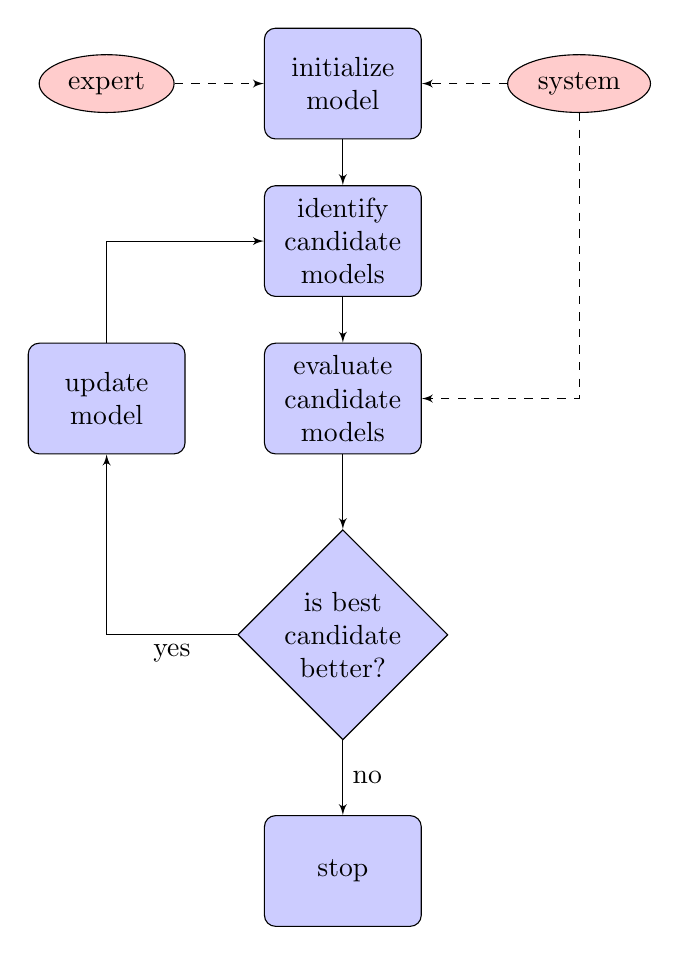
\begin{tikzpicture}[node distance = 2cm, auto]
    \tikzstyle{decision} = [diamond, draw, fill=blue!20,
    text width=4.5em, text badly centered, node distance=3cm, inner sep=0pt]
\tikzstyle{block} = [rectangle, draw, fill=blue!20,
    text width=5em, text centered, rounded corners, minimum height=4em]
\tikzstyle{line} = [draw, -latex']
\tikzstyle{cloud} = [draw, ellipse,fill=red!20, node distance=3cm,
minimum height=2em]

    % Place nodes
    \node [block] (init) {initialize model};
    \node [cloud, left of=init] (expert) {expert};
    \node [cloud, right of=init] (system) {system};
    \node [block, below of=init] (identify) {identify candidate models};
    \node [block, below of=identify] (evaluate) {evaluate candidate models};
    \node [block, left of=evaluate, node distance=3cm] (update) {update model};
    \node [decision, below of=evaluate] (decide) {is best candidate better?};
    \node [block, below of=decide, node distance=3cm] (stop) {stop};
    % Draw edges
    \path [line] (init) -- (identify);
    \path [line] (identify) -- (evaluate);
    \path [line] (evaluate) -- (decide);
    \path [line] (decide) -| node [near start] {yes} (update);
    \path [line] (update) |- (identify);
    \path [line] (decide) -- node {no}(stop);
    \path [line,dashed] (expert) -- (init);
    \path [line,dashed] (system) -- (init);
    \path [line,dashed] (system) |- (evaluate);
\end{tikzpicture}
\end{frame}

\begin{frame}[fragile]
  \frametitle{Monoids}
  \begin{tikzpicture}[node distance = 8mm, auto]
    \tikzstyle{box} = [rectangle, draw, text centered, rounded corners, minimum width=6mm, minimum height=6mm]
    \tikzstyle{line} = [draw, -latex']

    \node [box, draw=none] (a0) {};
    \node [box, fill=beamer@centricgreen!70, right of=a0] (a1) {h};
    \node [box, fill=beamer@codeblue!70, right of=a1] (a2) {e};
    \node [box, fill=beamer@centricgreen!70, right of=a2] (a3) {l};
    \node [box, fill=beamer@codeblue!70, right of=a3] (a4) {l};
    \node [box, fill=beamer@centricgreen!70, right of=a4] (a5) {o};
    \node [box, fill=beamer@codeblue!70, right of=a5] (a6) { };
    \node [box, fill=beamer@centricgreen!70, right of=a6] (a7) {w};
    \node [box, fill=beamer@codeblue!70, right of=a7] (a8) {o};
    \node [box, fill=beamer@centricgreen!70, right of=a8] (a9) {r};
    \node [box, fill=beamer@codeblue!70, right of=a9] (a10) {l};
    \node [box, fill=beamer@centricgreen!70, right of=a10] (a11) {d};
    \node [box, fill=beamer@codeblue!70, right of=a11] (a12) {!};

    \foreach \char/\pos in {h/1,e/2,l/3,l/4,o/5, /6,w/7,o/8,r/9,l/10,d/11,!/12} {
      \node [box, below of=a\pos] (b\pos) {\char};
      \path [line] (b\pos) -- (a\pos);
    }
\end{tikzpicture}
\end{frame}

\begin{frame}
  \frametitle{Calculating With Monoids}
  \begin{itemize}

  \item adding things (or multiplying)
  \item min and max
  \item map of key to value (for any monoid as value)
  \item ...
  \item we can calculate our metrics with monoids
  \item chars is the integer monoid with addition
  \item lines is also the integer monoid, but only count 1 if char is a newline
  \item for words, for now just split the input and count 1 on every ``group''
  \end{itemize}
\end{frame}

\begin{frame}
  \frametitle{Metrics With Monoids}
  \begin{itemize}
  \item calculate some metrics like: words, chars, lines
  \item some metrics cannot be expressed however
  \end{itemize}
\end{frame}

\begin{frame}
  \frametitle{You can nest monoids}
  \begin{itemize}
  \item monoids compose naturally
  \item handy because future of monoid is still a monoid
  \end{itemize}
\end{frame}

\begin{frame}
  \frametitle{Products of Monoids}
  \begin{itemize}
  \item a tuple of monoids is still a monoid, that works component wise
  \item handy for our case study!
  \end{itemize}
\end{frame}

\begin{frame}
  \frametitle{From Monoids To Applicatives}
  \begin{itemize}
  \item applicative functors are very similar to monoids
  \item monoidal in the effects (pure = ``empty'' effect, ap = ``effect chaining'')
  \end{itemize}
\end{frame}

\begin{frame}
  \frametitle{The Const Functor}
  \begin{itemize}
  \item the functor instance is a little strange
  \item but the applicative instance is super awesome
  \item allows you to lift any monoid into an applicative
  \item that means we can still use everything we already have
  \item (nb: Const is a monoid isomorphism)
  \end{itemize}
\end{frame}

\begin{frame}
  \frametitle{Metrics via Applicatives}
  \begin{itemize}
  \item using applicatives we have all the power we need
  \item use State, IO, Task, \ldots
  \end{itemize}
\end{frame}

\begin{frame}
  \frametitle{Brand New: Selective Functors}
  \begin{itemize}
  \item like applicatives, we can use a product of selective functors
  \item example: find the index of a word
  \end{itemize}
\end{frame}

\begin{frame}
  \frametitle{Using Foldable and Traverse}
  \begin{itemize}
  \item we can use Foldable and Traverse to abstract over the data structure
  \item both can also be composed!
  \end{itemize}
\end{frame}

\begin{frame}
  \frametitle{Okay but traversing Lists/Iterators/etc is suboptimal!}
  \begin{itemize}
  \item but there is no \texttt{traverse} for real streams?!
  \item because there can't be one\ldots
  \item but: do we need the actual \texttt{traverse}?
  \item realization: \texttt{traverse\_} is enough!
  \end{itemize}
\end{frame}

\begin{frame}
  \frametitle{Traverse and Foldable}
  \begin{itemize}
  \item so what's the difference between \texttt{traverse} and \texttt{traverse\_}
  \item the regular \texttt{traverse} keeps the whole structure!
  \item the \texttt{traverse\_} variant only secquences effects!
  \item and again: Applicative effect sequencing is associative (parallel!)
  \end{itemize}
\end{frame}

\begin{frame}
  \frametitle{Traversing with State}
  \begin{itemize}
  \item using State, we can still iterate imperatively
  \item but we can keep keep the parts separate and \textbf{compose} them!
  \item all the power from the normal imperative approach with all the benefits
  \end{itemize}
\end{frame}

\begin{frame}
  \frametitle{Traversing Streams}
  \begin{itemize}
  \item calculate length as well as do something
  \item log element and also write to db
  \item keep concerns separate and isolated
  \end{itemize}
\end{frame}

\begin{frame}
  \frametitle{Composition}
  \begin{itemize}
  \item use \texttt{Nested} to nest applicatives for ultimate power
  \item separate state update and retrieval + counting
  \item important gotcha: no real streaming depending on the applicative! (state...)
  \end{itemize}
\end{frame}

\begin{frame}
  \frametitle{The Tradeoffs}
  \begin{itemize}
  \item streaming is not possible with this approach, but only an example
  \item abstractions like Monoid and Applicative compose nicely
  \end{itemize}
\end{frame}

\begin{frame}
  \frametitle{Monadic composition?}
  \begin{itemize}
  \item monadic composition is not nearly as nice
  \item needs commutative monads
  \item see essence iterator 5.4
  \end{itemize}
\end{frame}

\section{Conclusion}\label{sec:conclusion}

\begin{frame}
  \frametitle{Conclusion}
  \begin{itemize}
  \item we can add metrics easily
  \item control flow can be easily customized
  \item (Sometimes) Monads are overrated
  \end{itemize}
\end{frame}

\appendix{}

\end{document}
